% Template-independent main body for the narrow STRI paper.
% Venue-specific preamble, author block, and bibliography style are intentionally external.
\begin{abstract}
Self-evolving language-model agents increasingly treat skill identities as control objects: a sampled skill can determine the next training task, a fresh ID can receive retrieval priority, and feedback can be written back to the selected package. We ask whether such control should change when the same semantic capabilities are merely split, cloned, or regrouped into different package identities. We formulate \emph{Skill-Taxonomy Representation Invariance} (STRI) and document identity sensitivity in two released self-evolving systems, Skill Self-Play (Skill-SP) and SkillRL. For a frozen context-by-package support matrix $A$, define $R^*(A)=\min_{w\ge0,t\ge0}\{t:\mathbf 1\le Aw\le t\mathbf 1\}$. We prove that $R^*=1$ iff nonnegative package weights can exactly equalize additive semantic exposure, derive the LP dual as a general lower-bound certificate, and show that the simple factor-2 singleton-overlap witness is one sparse dual solution. Skill-SP API-Bank Level-1 has $R^*=2$ on the full matrix, a frozen calibration subset, and a tool-disjoint heldout subset. Exhaustive one-cell stress tests preserve this positive residual under all 1,387 support additions and all 366 support deletions that keep the affected row covered. Two real negative regimes sharpen the boundary: Level-3 is disjoint and equalizable, while 127/128 logical-compiler tasks overlap yet $R^*=1$ because an umbrella package supports every row. That latter equality is concentrated rather than universally robust: a 75\% package-mass cap raises the constrained optimum to $4/3$, and 127/595 non-uncovering single-edge deletions break equalizability. Thus overlap prevalence is not the mechanism; the relevant object is support geometry together with the controller's feasible package-mass set. STRI-Cert operationalizes this as a fail-closed audit, with exact, dual, constrained, and box-robust variants. We do not claim LP algorithmic novelty or downstream harm: a faithful Qwen3-8B dynamic pilot failed qualification, while a separate qualified SkillRL bridge found no terminal-success disagreement beyond its matched identity placebo.
\end{abstract}

\section{Introduction}
Many self-evolving agents adapt through external state---memories, skills, workflows, tools, prompts, retrieval policies, or harness code---rather than only through foundation-model weights. Skills are especially attractive because a skill can package reusable procedure, metadata, examples, applicability information, and verification logic. Recent systems make the skill identity itself a control variable: Skill-SP~\citep{huang2026skill} samples a skill before generating a training task, while SkillRL~\citep{xia2026skillrl} gives dynamically created skill IDs priority in a fixed retrieval budget.

This architecture makes the \emph{representation} of the skill library consequential. Consider two taxonomies that expose the same executable semantic capability. One stores a primitive once; another stores an exact clone under a fresh ID. One represents generic and specific capabilities separately; another groups unchanged primitives behind a macro package. If no new primitive behavior or support region is added, should the future curriculum, retrieval exposure, or credit allocation change solely because package bookkeeping changed?

Existing work on semantic skill clones, redundancy governance, skill safety, adaptive routing, compression, and structured bandits establishes that skill quality, redundancy, and routing matter. These lines do not define a representation-invariance property for an endogenous evolution controller. We therefore ask: \emph{when can package-indexed control be made invariant to semantics-preserving changes in the skill taxonomy using the same frozen support information?}

We approach the question asset-first. Rather than proposing a normalization method and manufacturing a benchmark, we inspect released control surfaces, reduce the phenomenon against strongest same-information baselines, and identify a support geometry that separates positive and negative regimes.

\paragraph{Released Skill-SP.} On API-Bank Level-1, 314 released tasks are covered by at least one released validator and 183 have multiple memberships. The release's name+description Jaccard duplicate filter at threshold 0.33 misses all five observed specific--generic support-overlap pairs. Minimum-cardinality whole-package pruning can reduce the active library from 10 to 7 while preserving exact support, but 71 overlapping tasks remain. The residual is therefore not merely an exact-clone artifact.

\paragraph{Released SkillRL.} In released template-mode retrieval, dynamic general skills are included before the remaining fixed \texttt{top\_k=6} budget is filled with static skills. Adding one exact-content fresh-ID copy at a time admits all 12 tested clones. Across 223 released ALFWorld task descriptions, 11/12 clone targets change the unique semantic retrieval set and 5/12 reduce the number of unique general-skill contents returned.

These systems establish representation sensitivity, but not its mechanism. A natural hypothesis is simply that more overlap causes more sensitivity. Our main result rejects that hypothesis.

\paragraph{Contributions.}
\begin{enumerate}[leftmargin=*]
\item \textbf{STRI problem and released evidence.} We formulate representation invariance for skill-indexed self-evolution and document identity sensitivity in two independent released systems.
\item \textbf{Exact and dual certificates.} We derive $R^*(A)$, its exact LP dual, and a sparse factor-2 witness as a special dual certificate; we also give box-robust support and deployable max-share constrained variants without claiming a new optimization algorithm.
\item \textbf{Mechanism boundary and robustness.} Full, calibration, and tool-disjoint heldout Level-1 matrices have $R^*=2$ and survive exhaustive one-cell support perturbations; Level-3 and the high-overlap logical domain have $R^*=1$, while the logical result's dependence on an unrestricted umbrella weight is exposed by constrained auditing.
\item \textbf{Matched reductions and fail-closed audit.} STRI-Cert subsumes text/clone deduplication and whole-package pruning with the strongest same-information global reweighting, then reports exact, dual, quotient, sensitivity, and claim-boundary diagnostics without inferring downstream harm.
\end{enumerate}

\begin{figure}[t]
\centering
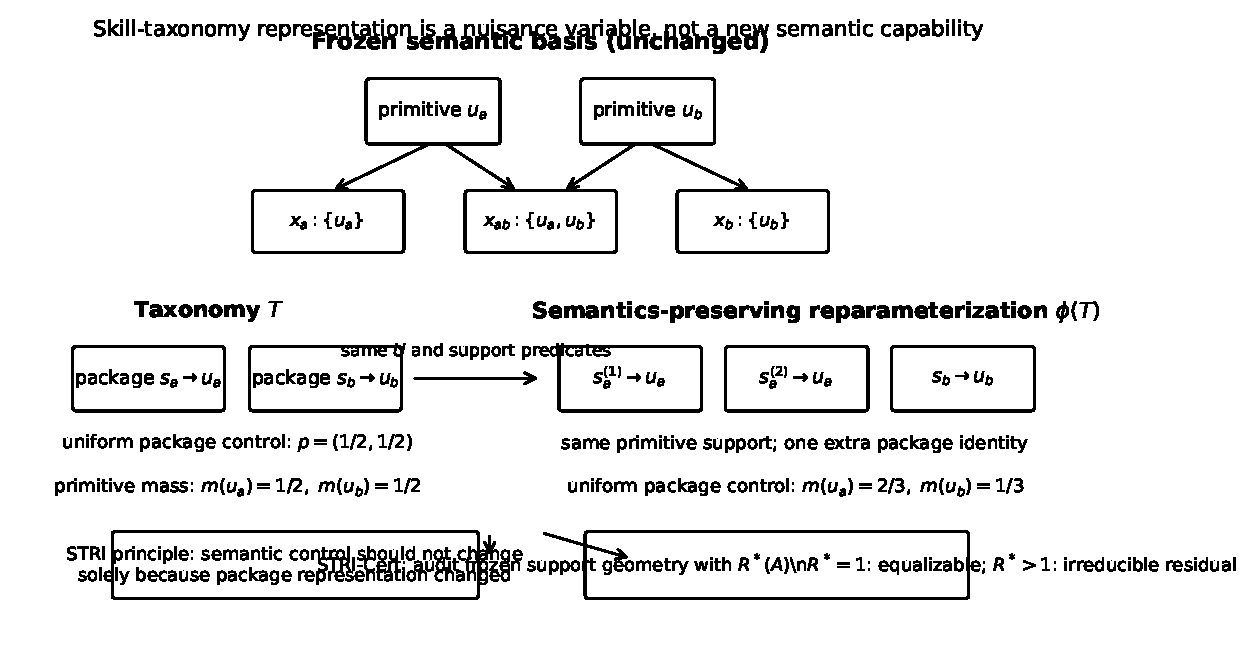
\includegraphics[width=0.98\linewidth]{figures/stri-overview.pdf}
\caption{STRI separates semantic capability from package representation. The conceptual identity-split example leaves the primitive basis and support predicates unchanged, yet a package-indexed controller can change primitive mass solely because one primitive has two package identities. Exact clones motivate the nuisance channel; the decisive released residual in Sec.~\ref{sec:evidence} survives clone reasoning and is characterized by non-equalizable partial-overlap support geometry.}
\label{fig:stri-overview}
\end{figure}

\section{From Package Identity to Semantic Exposure}
\label{sec:formalism}

\subsection{Frozen support matrix}
Let $X=\{x_1,\ldots,x_n\}$ be a finite set of semantic contexts or tasks with independently defined first-party support truth, and let $S=\{s_1,\ldots,s_m\}$ be the current skill packages. Define the binary incidence matrix
\[
A_{ij}=\mathbf{1}\{s_j\text{ supports }x_i\}.
\]
The support definition is frozen before evaluating STRI. In the tool-call study, support comes from released Skill-SP validators. In the logical-reasoning study, tasks are generated by released compiler specifications, checked by the author's fixed CSP/contract code, and cross-skill support is determined by the released compiler-alignment predicate.

We study package-only pre-context control. At a frozen state, the controller chooses nonnegative package mass $w\in\mathbb{R}^m_{\ge0}$ before the semantic task to be generated exists. The additive eligibility exposure of context $x_i$ is $e_i=(Aw)_i$. This is a control-opportunity quantity, not a task probability and not utility.

\subsection{Same-information pre-task controllers reduce to package mass}
In released Skill-SP, skill selection occurs before task generation. At this decision point the action is one current package identity. For any fixed pre-task state $z$, every randomized same-information rule---including a bandit, MLP, or neural router---induces a categorical distribution over packages, hence one nonnegative mass vector $w(z)$. The strongest same-information baseline is therefore arbitrary nonnegative package mass with access to the complete frozen support matrix.

This reduction is pointwise in $z$. It does \emph{not} claim that a longitudinal adaptive controller is globally equivalent to one static vector, and it does not allow a baseline to condition on the future generated task when the reviewed controller acts before that task exists.

\section{Exact Equalizability and STRI-Cert}
\label{sec:certificate}

\subsection{Exact finite-support criterion}
The max/min exposure ratio is invariant to positive scaling of $w$. We normalize every covered context to exposure at least one and define
\begin{equation}
\label{eq:rstar}
R^*(A)=\min_{w\ge0,\,t\ge0}t
\quad\text{s.t.}\quad
\mathbf 1\le Aw\le t\mathbf 1.
\end{equation}

\paragraph{Theorem 1 (finite-support package-only equalizability).}
$R^*(A)=1$ if and only if there exists a nonnegative package-only controller that gives exactly equal additive exposure to every covered context. If $R^*(A)>1$, no such package weighting exists, and $R^*(A)$ is the tight minimum achievable max/min exposure ratio.

\paragraph{Proof.}
If exact equalization exists, rescale its positive common exposure to one, giving a feasible solution with $t=1$. The constraints imply $t\ge1$, so $R^*(A)=1$. Conversely, $R^*(A)=1$ implies $\mathbf1\le Aw\le\mathbf1$, hence $Aw=\mathbf1$. For any $w$ with positive exposure on every covered row, let $r=\min_i(Aw)_i$ and rescale to $\tilde w=w/r$. Then $\min_i(A\tilde w)_i=1$ and the smallest feasible $t$ is $\max_i(Aw)_i/\min_i(Aw)_i$. Minimizing over $w$ yields exactly the tight multiplicative distortion. \hfill$\square$

The optimization itself is standard linear programming; the scientific object is the representation-invariance property that it decides.

\paragraph{Proposition 1 (dual certificate).}
The dual of Eq.~\eqref{eq:rstar} is
\begin{equation}
\label{eq:dual}
D^*(A)=\max_{\alpha,\beta\ge0}\mathbf1^\top\alpha
\quad\text{s.t.}\quad
A^\top(\beta-\alpha)\ge0,\quad \mathbf1^\top\beta\le1.
\end{equation}
Strong duality gives $D^*(A)=R^*(A)$. Thus every dual-feasible $(\alpha,\beta)$ is a certified lower bound, while an optimal pair is complete even when no local witness template is available. On every audited regime the numerical primal--dual gap is below $10^{-8}$.

\subsection{Human-readable factor-2 witness}
\paragraph{Theorem 2 (global-singleton overlap lower bound).}
Suppose packages $a,b$ each have a context supported by exactly that one package over the full frozen support universe, and another context is supported by both $a$ and $b$, possibly with additional packages. If both singleton contexts retain positive exposure, then every nonnegative package mass has max/min exposure ratio at least two on the focal rows, and therefore $R^*(A)\ge2$ for the full support matrix.

\paragraph{Proof.}
Let $r>0$ be the minimum exposure among the two singleton contexts and the shared context. Since the first singleton support signature is exactly $\{a\}$, its exposure is $w_a\ge r$; likewise $w_b\ge r$. The shared context contains both $a$ and $b$, and additional packages have nonnegative weight, so its exposure is at least $w_a+w_b\ge2r$. Thus every $w$ has focal max/min ratio at least two. For the same $w$, the full-matrix maximum is no smaller than the focal maximum and the full-matrix minimum is no larger than the focal minimum, so the full-matrix ratio is also at least two. Minimizing over $w$ gives $R^*(A)\ge2$. \hfill$\square$

Theorem~2 is also a sparse dual certificate: put $\alpha=1$ on the two singleton rows, $\beta=1$ on their shared row, and zero elsewhere. Dual feasibility follows from the support pattern and the objective is two. In released Skill-SP Level-1, the LP dual recovers exactly such a sparse optimum; the primal attains $R^*=2$, so the lower bound is tight.

\begin{figure}[t]
\centering
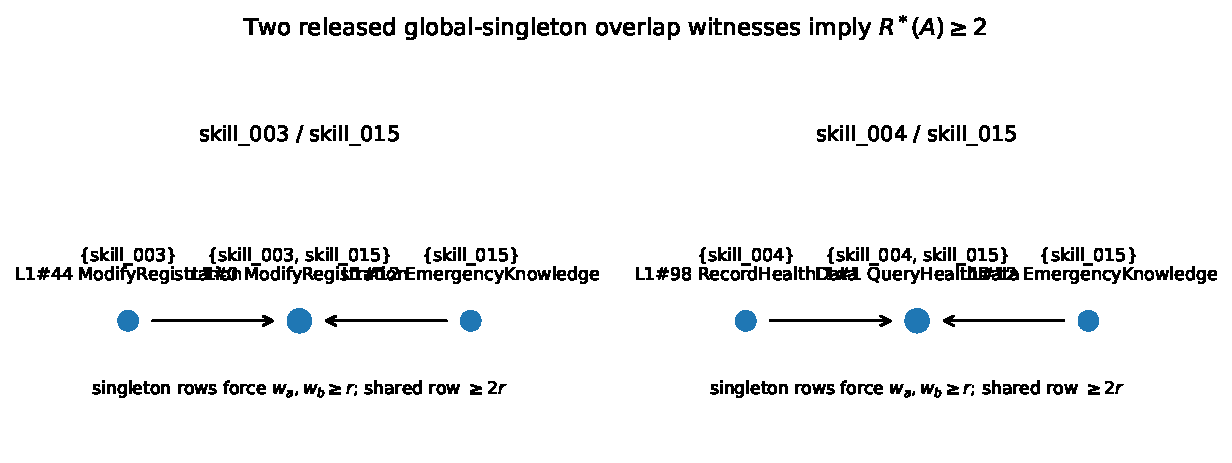
\includegraphics[width=0.96\linewidth]{figures/stri-factor2-witnesses.pdf}
\caption{Two released global-singleton overlap witnesses. In each case, retaining positive exposure on the two singleton regions forces at least twice that minimum exposure on the shared region.}
\label{fig:factor2-witnesses}
\end{figure}

\subsection{STRI-Cert and deployable variants}
STRI-Cert is a diagnostic protocol, not a learned predictor or a new LP solver: freeze independently defined support; solve Eq.~\eqref{eq:rstar} and its dual; report equalizable iff $R^*=1$, otherwise the tight residual; expose a sparse human-readable witness when one exists; and fail closed when support or optimization is invalid. Arbitrary nonnegative global package reweighting already receives the complete frozen support matrix, making text deduplication, clone removal, uniform routing, and scalar retuning weaker same-information reductions.

Two extensions make the assumptions explicit. First, for graded support with independently justified cellwise bounds $0\le L\le A\le U$ and nonnegative $w$, the exact box-robust audit is
\begin{equation}
\label{eq:robust}
R^*_{[L,U]}=\min_{w,t} t\quad\text{s.t.}\quad Lw\ge\mathbf1,\;Uw\le t\mathbf1,\;w,t\ge0,
\end{equation}
because the worst lower and upper additive exposures occur at $L$ and $U$. Estimating valid bounds remains a separate identification problem. Second, deployment constraints can be audited rather than ignored: adding $w_j\le\rho\sum_k w_k$ for every package defines a max-share constrained $R^*_{\rho}\ge R^*$. Both remain linear programs.

% Auto-generated from generated/asset-first-stri-narrow-paper-table-data-20260816.json.
% Narrow STRI submission tables. No dynamic/SQC success claims.

\begin{table}[t]
\centering
\caption{Released-system evidence for package-identity representation sensitivity. The two systems expose different control channels; only Skill-SP supplies the support matrix used by STRI-Cert.}
\label{tab:released-systems}
\small
\setlength{\tabcolsep}{4pt}
\begin{tabular}{p{0.20\linewidth}p{0.29\linewidth}p{0.43\linewidth}}
\toprule
System & Control surface & Released evidence \\
\midrule
Skill Self-Play (tool-call) & Pre-task skill sampling and skill-ID feedback/refinement & 183 multi-membership Level-1 rows among 314 covered rows; the released text duplicate filter misses all 5/5 observed specific--generic support-overlap pairs; exact-support whole-package pruning still leaves 71 overlap rows. \\
SkillRL & Fixed-budget template-mode dynamic skill retrieval & 12/12 exact-content fresh-ID clones are admitted; 11/12 clone targets change the unique semantic retrieval set over 223 released ALFWorld task descriptions; 5/12 reduce the number of unique general-skill contents. \\
\bottomrule
\end{tabular}
\end{table}

\begin{table}[t]
\centering
\caption{Reduction tournament on the Skill-SP tool-call support matrix. The strongest same-information reduction is arbitrary nonnegative global package weighting with access to the complete frozen support matrix.}
\label{tab:reductions}
\small
\setlength{\tabcolsep}{3.5pt}
\begin{tabular}{p{0.31\linewidth}p{0.20\linewidth}p{0.41\linewidth}}
\toprule
Reduction & Outcome & Evidence \\
\midrule
Released name+description Jaccard duplicate filter & Does not absorb & Misses all 5/5 observed specific--generic support-overlap pairs; similarity 0.1429--0.20 is below the released 0.33 threshold. \\
Exact semantic-clone deduplication & Does not absorb partial overlap & The positive regime uses distinct specific/generic packages with different unique support regions. \\
Minimum-cardinality whole-package pruning preserving exact support & Partial reduction only & Active packages drop from 10 to 7, but 71 overlap rows remain while exact support is preserved. \\
Arbitrary nonnegative global package weights & Exact residual & The exact optimum is $R^*(A)=2$. \\
Global-singleton overlap witness & Closed-form lower bound & Two independent released witnesses imply $R^*(A)\ge 2$, and the exact LP attains 2. \\
\bottomrule
\end{tabular}
\end{table}

\begin{table}[t]
\centering
\caption{Mechanism boundary across real first-party support regimes. High overlap is neither necessary nor sufficient for an irreducible package-only residual; the exact discriminator is $R^*(A)$.}
\label{tab:support-boundary}
\small
\setlength{\tabcolsep}{3.2pt}
\begin{tabular}{p{0.34\linewidth}rrrrp{0.18\linewidth}}
\toprule
Regime & Covered & Multi & Overlap & $R^*$ & Certificate \\
\midrule
API-Bank Level-1 full & 314 & 183 & 58.3\% & 2.0 & Residual \\
Level-1 calibration tools & 47 & 33 & 70.2\% & 2.0 & Residual \\
Level-1 tool-disjoint heldout & 52 & 38 & 73.1\% & 2.0 & Residual \\
API-Bank Level-3 & 34 & 0 & 0.0\% & 1.0 & Equalizable \\
Logical compiler validation & 128 & 127 & 99.2\% & 1.0 & Equalizable \\
\bottomrule
\end{tabular}
\end{table}

\begin{table}[t]
\centering
\caption{Preregistered faithful Qwen3-8B dynamic pilot. Qualification is checked before any dynamic STRI witness may update scientific belief.}
\label{tab:qwen-p0a}
\small
\begin{tabular}{lrrr}
\toprule
Source skill & Generated & Contract-valid & Required \\
\midrule
skill\_003 & 24 & 14 & 16 \\
skill\_004 & 24 & 5 & 16 \\
skill\_015 & 24 & 8 & 16 \\
\bottomrule
\end{tabular}
\vspace{2pt}

\footnotesize Formal outcome: \texttt{INCONCLUSIVE\_\allowbreak PROPOSER\_\allowbreak QUALIFICATION\_\allowbreak FAILED}. The 72-generation bank supplies no dynamic STRI belief update and is not rerun.
\end{table}


\begin{figure}[t]
\centering
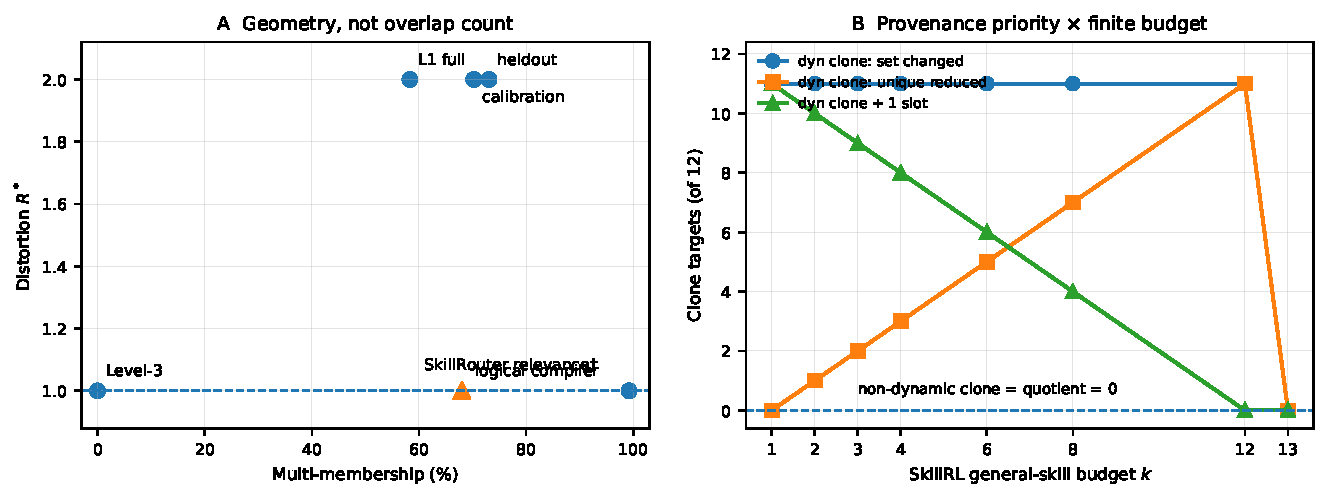
\includegraphics[width=0.82\linewidth]{figures/stri-rstar-boundary.pdf}
\caption{Overlap prevalence does not determine STRI residual. The three Level-1 regimes independently have $R^*(A)=2$, while Level-3 is equalizable with disjoint support and the logical compiler domain is equalizable despite 127/128 multi-membership tasks.}
\label{fig:rstar-boundary}
\end{figure}

\section{Released-System Evidence}
\label{sec:evidence}

\subsection{Skill-SP tool-call support: positive regime}
On API-Bank Level-1, 314 rows are accepted by at least one released Skill-SP validator and 183 have multiple memberships. STRI-Cert gives $R^*=2.0$.

To test whether this is an artifact of fitting package weights to the complete table, we use a tool-disjoint split frozen before the later certificate analysis. Calibration uses \texttt{AppointmentRegistration}, \texttt{ModifyRegistration}, \texttt{QueryHealthData}, and \texttt{RecordHealthData}; heldout uses \texttt{CancelRegistration}, \texttt{EmergencyKnowledge}, \texttt{QueryRegistration}, and \texttt{SymptomSearch}. Calibration has 47 covered tasks, 33 multi-membership rows, and $R^*=2$. Heldout has 52 covered tasks, 38 multi-membership rows, and again $R^*=2$. Both independently contain the two globally valid factor-2 witness structures.

The witness rows are directly inspectable. For \texttt{skill\_003}/\texttt{skill\_015}, L1\#44 and L1\#12 are singleton regions while L1\#0 is shared. For \texttt{skill\_004}/\texttt{skill\_015}, L1\#98 and L1\#12 are singleton regions while L1\#1 is shared. In each case Theorem~2 yields the same lower bound attained by the exact LP.

\subsection{Level-3: disjoint-support negative control}
Level-3 provides a natural released negative regime. Thirty-four rows are covered, every covered row has exactly one skill membership, and $R^*=1$. Equal weights on the active packages equalize every covered task. STRI-Cert therefore does not mechanically label every released taxonomy problematic.

\subsection{Logical compiler domain: high overlap but no residual}
A stronger negative test asks whether high overlap alone triggers the certificate. Skill-SP's logical-reasoning release contains eight skill packages with programmatic compiler specifications. The author code can generate a zebra puzzle from a compiler, verify it with a fixed CSP solver, and check whether a generated sample satisfies each package's released compiler-alignment contract.

We freeze the author's default compiler-validation sizes $(3\!\times\!3,4\!\times\!4,5\!\times\!5,6\!\times\!6)$ and seeds $0,1,2,3$ for each of eight released skills, giving 128 source units. No language model is used. All 128/128 units compile and pass the author's puzzle contract and uniqueness verifier; every task is then cross-evaluated against all eight released support specifications.

The support matrix is extremely overlapping: 127/128 tasks have more than one supported skill, with 38 distinct support patterns. Yet $R^*=1$. The exact LP places all mass on \texttt{skill\_008}, whose released alignment contract supports every generated unit. This is a valid but concentrated equalizer. Under the practical max-share constraint above, $R^*_{0.75}=4/3$, $R^*_{0.5}=2$, and $R^*_{0.25}=4$. Thus the umbrella is not silently treated as universally benign: it identifies the precise feasible-set assumption under which this high-overlap regime is equalizable.

The mechanism is therefore not ``more overlap implies more representation dependence.'' It is whether support geometry admits an equalizer \emph{within the controller's declared feasible package-mass set}.

\subsection{SkillRL: phenotype first, certificate only with independent support}
SkillRL shows that identity sensitivity is not confined to one implementation. In released template-mode retrieval, fresh dynamic IDs receive priority in a fixed general-skill budget. Exact-content fresh-ID clones are admitted for all 12 tested skills; 11/12 clone targets change the unique semantic retrieval set over 223 ALFWorld descriptions, and 5/12 reduce its unique-content count under \texttt{top\_k=6}.

We deliberately separate two audit stages. Identity perturbation can be tested directly from SkillRL's released retrieval behavior, but $R^*$ requires an independently defined context-by-package support matrix. SkillRL does not expose the first-party support contract needed for that second stage, so we do \emph{not} retrofit a learned, candidate-defined $A$ merely to make the certificate run. Skill-SP supplies such contracts and therefore supports the mechanistic certificate. Section~\ref{sec:dynamic} separately tests whether the SkillRL retrieval phenotype reaches terminal success.

\subsection{Matched baselines, representation ablations, and failure analysis}
Table~\ref{tab:reductions} is an explicit same-information baseline ladder, not a collection of unrelated heuristics. The first three baselines may inspect the same complete released support object but can only remove duplicate package columns or whole packages. Minimum exact-coverage pruning is already strong: it removes 61.2\% of the observed Level-1 overlap (183 to 71 multi-membership rows). Yet the residual survives. The strongest context-independent baseline then receives arbitrary nonnegative package weights and the full support matrix; its exact optimum remains $R^*=2$ on the full, calibration, and heldout Level-1 regimes. This is the point at which a simpler package-level explanation is exhausted.

We next ablate the representation itself (Figure~\ref{fig:ablation-robustness}A). Each active Level-1 package is cloned and split independently while preserving its support column. These interventions deliberately perturb package multiplicity without adding a support region. Before quotienting, cloning \texttt{skill\_003}, \texttt{skill\_004}, or the generic \texttt{skill\_015} changes the two-witness closed-form diagnostic to 1, 1, and 0 witnesses respectively. This is not a change in the exact certificate: duplicating a support column leaves $R^*$ unchanged because duplicate weights can be merged or one duplicate can receive zero mass. It instead exposes an implementation pitfall in the human-readable witness search. Exact-support quotienting removes the nuisance duplication and recovers every original support row and both witnesses for every clone and split control. A bijective renaming of all package IDs leaves the diagnostics unchanged. Thus the quotient is not cosmetic; it is required for the interpretable witness layer to inherit the representation invariance of the exact LP.

Finally, we locate both witness and support sensitivity. Across 49 Level-1 tools, 4 have a closed-form witness, 10 have overlap without that template, 20 are disjoint/singleton-only, and 15 have no support (Figure~\ref{fig:ablation-robustness}C). The exact per-tool LP resolves all 10 overlap-without-witness cases as $R^*=1$; all four tool-local residuals are caught by the sparse witness. This does not make Theorem~2 complete in general---Eq.~\eqref{eq:dual} is the authority when the obstruction is nonlocal.

The aggregate positive result is substantially more stable than mere witness resampling suggests. Exhaustively flipping every single zero support cell to one gives 1,387 perturbed Level-1 matrices, all still residual ($R^*\in[2,3]$). Removing each support edge that leaves its row covered gives 366 more matrices, all with $R^*=2$; 131 deletions that would uncover a row fail closed. The negative boundaries reveal the opposite asymmetry: every one of 102 possible Level-3 support additions changes $R^*=1$ to $2$, while the logical domain survives all 428 additions but only 468/595 non-uncovering deletions (127 break equalizability). These are exact one-cell finite-snapshot stress tests, not a claim that a learned support estimator is calibrated or that arbitrary multi-cell noise is harmless. The earlier leave-one-tool/row and 500 fixed-seed tool-bootstrap tests remain consistent: both Level-1 witnesses survive every deletion; at least one survives 100\% and both 97.2\% of bootstrap replicates.

\begin{figure}[t]
\centering
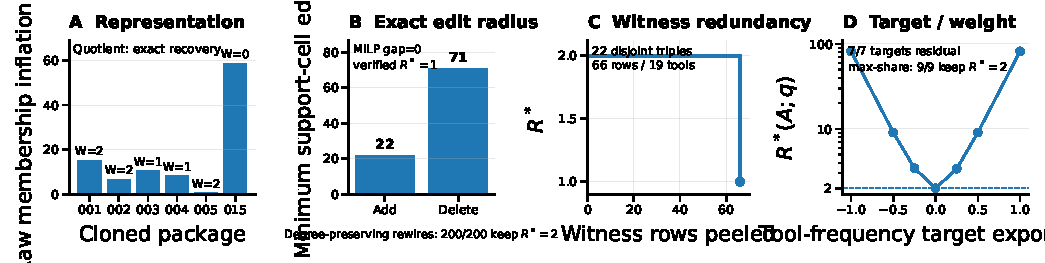
\includegraphics[width=0.99\linewidth]{figures/stri-ablation-robustness.pdf}
\caption{Representation-ablation and robustness evidence. \textbf{A:} clone-induced raw multiplicity/witness changes vanish under exact-support quotienting. \textbf{B:} factor-2 witnesses survive deletion tests and 500 tool resamples. \textbf{C:} the simple witness is only a template; exact LP subsequently resolves the ten overlap/no-witness tools as equalizable.}
\label{fig:ablation-robustness}
\end{figure}

\section{Relation to Existing Work}
\label{sec:related}

\paragraph{Skill redundancy and clone detection.}
Prior work studies semantic skill clones, duplicate propagation, and clone-aware filtering~\citep{zhu2026skillclone}. STRI therefore does not claim that duplicate skills exist or that exact duplicates should be detected. The focal positive regime survives exact-clone reasoning because specific and generic packages have distinct unique support regions in addition to shared contexts.

\paragraph{Redundancy-aware lifecycle governance.}
Prior governance methods recommend, attribute, suppress, merge, or update redundant and environment-sensitive skills~\citep{liu2026skillsvote}. Such policies may improve performance, but they do not answer whether a frozen taxonomy admits representation-invariant package-only control. STRI-Cert is a property test of control/support geometry rather than a competing recommendation algorithm.

\paragraph{Skill safety and failures.}
Work on unsafe skill evolution and harmful agent skills demonstrates that learned or retrieved skill content can propagate functional or efficiency failures~\citep{mao2026practiceunsafe,dong2026agentskills}. Our primary support transformations keep the audited semantic support predicates fixed. A positive STRI certificate does not imply unsafe content or downstream failure.

\paragraph{Adaptive routing and evolving skills.}
ERSkill, Skill-SP, SkillRL, SHAPER, and related systems learn routers or co-evolve skill libraries~\citep{chen2026erskill,huang2026skill,xia2026skillrl,wang2026shaper}. These works absorb any generic claim that adaptive routing or skill evolution is novel. They motivate STRI because package identities become endogenous actions or state, but they do not test invariance under a semantics-preserving reparameterization of that representation.

\paragraph{Compression, online learning, and classical balancing.}
Skill compression factors repeated procedure~\citep{bai2026skillzip}, while structured bandit/expert methods share information across related actions~\citep{slivkins2011contextual,sen2018stochastic}. Eq.~\eqref{eq:rstar} is also adjacent to classical fractional covering, matrix scaling, max--min fairness, and discrepancy/balancing~\citep{lovasz1975fractional,sinkhorn1967nonnegative,radunovic2007fairness,beck1981integer}. We do not claim these optimization ideas: fractional cover minimizes set cost under coverage, matrix scaling targets prescribed marginals, fairness orders resource allocations, and discrepancy typically balances signed/integer assignments. STRI instead uses nonnegative package mass to \emph{test invariance to taxonomy reparameterization} in an endogenous skill controller.

\section{Dynamic Boundary Tests}
\label{sec:dynamic}

Static exposure need not propagate to task utility, so we preregistered two bridges. A faithful Qwen3-8B Skill-SP pilot fixed skills 003/004/015, 24 generations each, released-style decoding, and at least 16 author-contract-valid tasks per source before any dynamic statistic was admissible. All 72 generations completed, but validity was only 14/24, 5/24, and 8/24; the frozen qualification gate therefore failed. We neither lowered it nor added generations, changed decoding, or switched backbone, and make no dynamic claim from this bank.

A separate SkillRL fixed-task bridge \emph{did} qualify: the author's final ALFWorld policy reached 18/24 competence-stage successes, followed by 24 paired A/B/C/D causal units. Every arm again had 18/24 terminal successes with zero paired endpoint disagreements. Exact-clone displacement B changed action trajectories in 11/24 units, versus 15/24 for the matched identity placebo C; exact quotienting D restored A trajectories in 24/24. Thus representation can alter retrieval and trajectories without a demonstrated terminal-success effect in this qualified realization. Because no equivalence margin or task-cluster power analysis was preregistered, this is a realization STOP, not a population-level no-effect theorem.

\section{Discussion and Claim Boundary}
\label{sec:discussion}

STRI-Cert answers a specification question before asking about utility: given independently defined finite support and a declared package-mass action class, can additive semantic exposure be equalized? $R^*>1$ proves that no controller in that class can remove the audited representation residual; it does not imply that the residual is harmful. $R^*=1$ proves only existence of an equalizer, not that the released controller uses it. The constrained $R^*_{\rho}$ further shows that ``equalizable'' is meaningful only relative to a declared feasible set.

The logical domain makes this distinction concrete. Its 99.2\% overlap looks more severe by redundancy count, yet unrestricted $R^*=1$ because an umbrella package covers every row; the same support becomes non-equalizable under modest anti-concentration constraints. Conversely, the Level-1 residual survives every single-edge addition and every deletion that leaves the affected row covered. A scalar overlap statistic cannot express either boundary.

The narrow claims are intentionally smaller than our original dynamic design. We \textbf{do} claim that released control surfaces can depend on skill-package representation, that $R^*(A)$ exactly characterizes package-only additive exposure equalizability on a frozen finite support matrix, and that the audited residual tracks support geometry rather than overlap prevalence. We \textbf{do not} claim that a positive certificate causes task failure, that static exposure predicts longitudinal utility, that STRI-Cert is computationally novel relative to linear programming, that high overlap is harmful in general, that Support-Quotient Control has been empirically validated, that the unqualified Qwen3 bank provides dynamic evidence, or that the qualified SkillRL bridge STOP proves population-level absence of a downstream effect.

A representation-invariant design would factor control through semantic support cells first, then distribute each cell's conserved mass among packages that implement it. Exact cloning would then change implementation responsibility but not semantic-cell mass. This recipe requires trustworthy support contracts and may face a combinatorial cell space; we therefore present it as a design consequence, not a validated utility method. Overall, STRI-Cert isolates support geometry and controller feasibility---not overlap prevalence---without conflating exposure with utility.

\section{Limitations}
\begin{enumerate}[leftmargin=*]
\item \textbf{Support identification.} Exact STRI needs independently defined support. Eq.~\eqref{eq:robust} propagates valid cellwise uncertainty bounds, and our one-cell audit measures local sensitivity, but neither solves the separate problem of learning calibrated support nor certifies arbitrary multi-cell error.
\item \textbf{Static exposure is not utility.} $R^*$ does not establish regret or end-of-evolution harm; the qualified SkillRL bridge is negative at terminal success in its tested realization.
\item \textbf{Finite domain and feasible set.} Certificates are exact only on audited contexts and the declared controller class. Post-context or support-cell controllers may avoid the package-only channel; practical weight restrictions can instead be represented by $R^*_{\rho}$ or other linear constraints.
\item \textbf{Dynamic evidence remains bounded.} The Skill-SP Qwen3 pilot failed its preregistered proposer gate, while the SkillRL bridge was not powered as an equivalence study. Neither licenses a population-level dynamic conclusion.
\end{enumerate}
